\documentclass[hyperref, a4paper, UTF8, zihao = -4, linespread = 1]{ctexbook}
\usepackage{lmodern}
\usepackage{amssymb,amsmath}
\usepackage{ifxetex,ifluatex}
\usepackage{fixltx2e} % provides \textsubscript
\ifnum 0\ifxetex 1\fi\ifluatex 1\fi=0 % if pdftex
  \usepackage[T1]{fontenc}
  \usepackage[utf8]{inputenc}
\else % if luatex or xelatex
  \ifxetex
    \usepackage{xltxtra,xunicode}
  \else
    \usepackage{fontspec}
  \fi
  \defaultfontfeatures{Ligatures=TeX,Scale=MatchLowercase}
\fi
% use upquote if available, for straight quotes in verbatim environments
\IfFileExists{upquote.sty}{\usepackage{upquote}}{}
% use microtype if available
\IfFileExists{microtype.sty}{%
\usepackage{microtype}
\UseMicrotypeSet[protrusion]{basicmath} % disable protrusion for tt fonts
}{}
\usepackage[a4paper,tmargin=2cm,bmargin=2cm,lmargin=2.5cm,rmargin=2cm]{geometry}
\usepackage[unicode=true]{hyperref}
\PassOptionsToPackage{usenames,dvipsnames}{color} % color is loaded by hyperref
\hypersetup{
            pdftitle={分析报告},
            pdfauthor={张三},
            colorlinks=true,
            linkcolor=Maroon,
            citecolor=Blue,
            urlcolor=Blue,
            breaklinks=true}
\urlstyle{same}  % don't use monospace font for urls
\usepackage{natbib}
\bibliographystyle{apalike}
\usepackage{color}
\usepackage{fancyvrb}
\newcommand{\VerbBar}{|}
\newcommand{\VERB}{\Verb[commandchars=\\\{\}]}
\DefineVerbatimEnvironment{Highlighting}{Verbatim}{commandchars=\\\{\}}
% Add ',fontsize=\small' for more characters per line
\usepackage{framed}
\definecolor{shadecolor}{RGB}{248,248,248}
\newenvironment{Shaded}{\begin{snugshade}}{\end{snugshade}}
\newcommand{\AlertTok}[1]{\textcolor[rgb]{0.94,0.16,0.16}{#1}}
\newcommand{\AnnotationTok}[1]{\textcolor[rgb]{0.56,0.35,0.01}{\textbf{\textit{#1}}}}
\newcommand{\AttributeTok}[1]{\textcolor[rgb]{0.77,0.63,0.00}{#1}}
\newcommand{\BaseNTok}[1]{\textcolor[rgb]{0.00,0.00,0.81}{#1}}
\newcommand{\BuiltInTok}[1]{#1}
\newcommand{\CharTok}[1]{\textcolor[rgb]{0.31,0.60,0.02}{#1}}
\newcommand{\CommentTok}[1]{\textcolor[rgb]{0.56,0.35,0.01}{\textit{#1}}}
\newcommand{\CommentVarTok}[1]{\textcolor[rgb]{0.56,0.35,0.01}{\textbf{\textit{#1}}}}
\newcommand{\ConstantTok}[1]{\textcolor[rgb]{0.00,0.00,0.00}{#1}}
\newcommand{\ControlFlowTok}[1]{\textcolor[rgb]{0.13,0.29,0.53}{\textbf{#1}}}
\newcommand{\DataTypeTok}[1]{\textcolor[rgb]{0.13,0.29,0.53}{#1}}
\newcommand{\DecValTok}[1]{\textcolor[rgb]{0.00,0.00,0.81}{#1}}
\newcommand{\DocumentationTok}[1]{\textcolor[rgb]{0.56,0.35,0.01}{\textbf{\textit{#1}}}}
\newcommand{\ErrorTok}[1]{\textcolor[rgb]{0.64,0.00,0.00}{\textbf{#1}}}
\newcommand{\ExtensionTok}[1]{#1}
\newcommand{\FloatTok}[1]{\textcolor[rgb]{0.00,0.00,0.81}{#1}}
\newcommand{\FunctionTok}[1]{\textcolor[rgb]{0.00,0.00,0.00}{#1}}
\newcommand{\ImportTok}[1]{#1}
\newcommand{\InformationTok}[1]{\textcolor[rgb]{0.56,0.35,0.01}{\textbf{\textit{#1}}}}
\newcommand{\KeywordTok}[1]{\textcolor[rgb]{0.13,0.29,0.53}{\textbf{#1}}}
\newcommand{\NormalTok}[1]{#1}
\newcommand{\OperatorTok}[1]{\textcolor[rgb]{0.81,0.36,0.00}{\textbf{#1}}}
\newcommand{\OtherTok}[1]{\textcolor[rgb]{0.56,0.35,0.01}{#1}}
\newcommand{\PreprocessorTok}[1]{\textcolor[rgb]{0.56,0.35,0.01}{\textit{#1}}}
\newcommand{\RegionMarkerTok}[1]{#1}
\newcommand{\SpecialCharTok}[1]{\textcolor[rgb]{0.00,0.00,0.00}{#1}}
\newcommand{\SpecialStringTok}[1]{\textcolor[rgb]{0.31,0.60,0.02}{#1}}
\newcommand{\StringTok}[1]{\textcolor[rgb]{0.31,0.60,0.02}{#1}}
\newcommand{\VariableTok}[1]{\textcolor[rgb]{0.00,0.00,0.00}{#1}}
\newcommand{\VerbatimStringTok}[1]{\textcolor[rgb]{0.31,0.60,0.02}{#1}}
\newcommand{\WarningTok}[1]{\textcolor[rgb]{0.56,0.35,0.01}{\textbf{\textit{#1}}}}
\usepackage{longtable,booktabs}
% Fix footnotes in tables (requires footnote package)
\IfFileExists{footnote.sty}{\usepackage{footnote}\makesavenoteenv{long table}}{}
\IfFileExists{parskip.sty}{%
\usepackage{parskip}
}{% else
\setlength{\parindent}{0pt}
\setlength{\parskip}{6pt plus 2pt minus 1pt}
}
\setlength{\emergencystretch}{3em}  % prevent overfull lines
\providecommand{\tightlist}{%
  \setlength{\itemsep}{0pt}\setlength{\parskip}{0pt}}
\setcounter{secnumdepth}{5}
% Redefines (sub)paragraphs to behave more like sections
\ifx\paragraph\undefined\else
\let\oldparagraph\paragraph
\renewcommand{\paragraph}[1]{\oldparagraph{#1}\mbox{}}
\fi
\ifx\subparagraph\undefined\else
\let\oldsubparagraph\subparagraph
\renewcommand{\subparagraph}[1]{\oldsubparagraph{#1}\mbox{}}
\fi

% set default figure placement to htbp
\makeatletter
\def\fps@figure{htbp}
\makeatother

\usepackage{booktabs}
\usepackage{longtable}


\usepackage{array}
\usepackage{multirow}
\usepackage{wrapfig}
\usepackage{float}
\usepackage{colortbl}
\usepackage{pdflscape}
\usepackage{tabu}
\usepackage{threeparttable}
\usepackage{threeparttablex}
\usepackage[normalem]{ulem}
\usepackage{makecell}
\usepackage{xcolor}
\usepackage{indentfirst}\setlength{\parindent}{2em}
\usepackage{setspace}\doublespacing


%%%%%%%%%%%%%%%%%%%%%%%%%%%%%%%%%%%%%%%%%%%%%%%%%%%%%%%%%%%%%
%\setCJKmainfont[
%     BoldFont=方正黑体简体,
%   ItalicFont=方正精楷简体,
%  SlantedFont=方正仿宋简体,
%]{方正黑体简体}

%\setCJKsansfont[
%     BoldFont=方正黑体简体,
%   ItalicFont=方正精楷简体,
%  SlantedFont=方正仿宋简体,
%]{方正中等线简体}

%\setCJKmonofont[
%     BoldFont=方正黑体简体,
%   ItalicFont=方正精楷简体,
%  SlantedFont=方正仿宋简体,
%]{方正精楷简体}


\newCJKfontfamily{\song}{SimSun}
\newCJKfontfamily{\hei}{SimHei}
\newCJKfontfamily{\fzxbsj} {方正小标宋简体}
\newCJKfontfamily{\fzfangsong}{方正仿宋简体}
\newCJKfontfamily{\fzheiti}{方正黑体简体}
\newCJKfontfamily{\fzjk}{方正精楷简体}
\newCJKfontfamily{\fzcusong} {方正粗宋简体}
\newCJKfontfamily{\fzzhysong}{方正中雅宋_GBK}
\newCJKfontfamily{\fzydzhhei}{方正韵动中黑简体}
\newCJKfontfamily{\fzliukai} {方正苏新诗柳楷简体}
%%%%%%%%%%%%%%%%%%%%%%%%%%%%%%%%%%%%%%%%%%%%%%%%%%%%%%%%%%%%%

\usepackage{framed,color}
\definecolor{shadecolor}{RGB}{248,248,248}

\renewcommand{\textfraction}{0.05}
\renewcommand{\topfraction}{0.8}
\renewcommand{\bottomfraction}{0.8}
\renewcommand{\floatpagefraction}{0.75}

\let\oldhref\href
\renewcommand{\href}[2]{#2\footnote{\url{#1}}}

\makeatletter
\newenvironment{kframe}{%
\medskip{}
\setlength{\fboxsep}{.8em}
 \def\at@end@of@kframe{}%
 \ifinner\ifhmode%
  \def\at@end@of@kframe{\end{minipage}}%
  \begin{minipage}{\columnwidth}%
 \fi\fi%
 \def\FrameCommand##1{\hskip\@totalleftmargin \hskip-\fboxsep
 \colorbox{shadecolor}{##1}\hskip-\fboxsep
     % There is no \\@totalrightmargin, so:
     \hskip-\linewidth \hskip-\@totalleftmargin \hskip\columnwidth}%
 \MakeFramed {\advance\hsize-\width
   \@totalleftmargin\z@ \linewidth\hsize
   \@setminipage}}%
 {\par\unskip\endMakeFramed%
 \at@end@of@kframe}
\makeatother

\makeatletter
\@ifundefined{Shaded}{
}{\renewenvironment{Shaded}{\begin{kframe}}{\end{kframe}}}
\@ifpackageloaded{fancyvrb}{%
  % https://github.com/CTeX-org/ctex-kit/issues/331
  \RecustomVerbatimEnvironment{Highlighting}{Verbatim}{commandchars=\\\{\},formatcom=\xeCJKVerbAddon}%
}{}
\makeatother

\usepackage{makeidx}
\makeindex

\urlstyle{tt}

\usepackage{amsthm}
\makeatletter
\def\thm@space@setup{%
  \thm@preskip=8pt plus 2pt minus 4pt
  \thm@postskip=\thm@preskip
}
\makeatother


%%%%%%%%%%%%%%%%%%%%%%%%%%%%%%%%%%%%%%%%%%%%%%%%%%%%%%%%%%%%%%%%%%%%%%%%%%%%%%%%%%%
\newcommand\chaptertitleformat[1]{%% 设置条件语句,如果是无编号标题就再加一条横线
    \ifthechapter{#1}{#1\medskip\hrule\medskip}}

\makeatletter
\newcommand*\thechapteron{\global\let\ifthechapter\@firstoftwo}
\newcommand*\thechapteroff{\global\let\ifthechapter\@secondoftwo}
\thechapteroff
\makeatother



\ctexset{
    chapter = {
        format      = \fzzhysong\LARGE\bfseries,
        nameformat  = \thechapteron,                  %% 切换 \ifthechapter
        aftername   = \medskip\hrule\medskip,         %% 有编号标题的横线
        titleformat = \raggedleft\chaptertitleformat, %% 右对齐,无编号标题下再加横线
        aftertitle  = \thechapteroff
    },
    section = {
        format = \zihao{3}\raggedright\Large\bfseries,
    }
}

% caption settings
\usepackage[font=small,labelfont={bf}]{caption}
\captionsetup[table]{skip=3pt}
\captionsetup[figure]{skip=3pt}
%%%%%%%%%%%%%%%%%%%%%%%%%%%%%%%%%%%%%%%%%%%%%%%%%%%%%%%%%%%%%%%%%%%%%%%%%%%%%%%%%%%


\frontmatter
\usepackage{booktabs}
\usepackage{longtable}
\usepackage{array}
\usepackage{multirow}
\usepackage{wrapfig}
\usepackage{float}
\usepackage{colortbl}
\usepackage{pdflscape}
\usepackage{tabu}
\usepackage{threeparttable}
\usepackage{threeparttablex}
\usepackage[normalem]{ulem}
\usepackage{makecell}
\usepackage{xcolor}

\title{分析报告}
\providecommand{\subtitle}[1]{}
\subtitle{优雅的 Bookdown 书籍模版}
\author{张三}
\date{2020-02-03}

\begin{document}
\maketitle


\thispagestyle{empty}

\begin{center}
%献给……

%呃,爱谁谁吧
\end{center}

\setlength{\abovedisplayskip}{-5pt}
\setlength{\abovedisplayshortskip}{-5pt}

{
\setcounter{tocdepth}{2}
\tableofcontents
}
\mainmatter

\hypertarget{intro}{%
\chapter{导言}\label{intro}}

2018年12月教育部等九部门印发中小学生减负措施的通知,要求切实减轻违背教育教学规律、有损中小学生身心健康的过重学业负担,促进中小学生健康成长,培养德智体美劳全面发展的社会主义建设者和接班人。我区坚持学生课业负担年度调查,了解相关减负政策的落实情况。2019年6月,对全区四、五、七年级的学生进行了学生课业负担状况问卷调查,分别收到有效数据7912、8018、5146份。本次学生课业负担状况主要考查学生的课业负担状况(包括客观课业负担和主观学习感受)和相关影响因素。通过主客观负担和影响因素数据的呈现,以及分析课业负担、学习方法、学习成绩三者的关联,进一步分析落实减轻学生学业负担、提高学生学习深度的有效路径。

本站《成语故事》收录了五千多个经典成语故事,如八仙过海、画龙点睛、守株待兔、一箭双雕等,都是我们耳熟能详的。成语故事按成语首字读音顺序排列,以故事形式对成语的出处、典故、含义进行清晰明了的解释,故事通俗易懂、内涵深刻、妙趣无穷,真实地再现了一段段传奇往事和历史遗痕。

\hypertarget{ux7b2cux4e00ux8282}{%
\section{第一节}\label{ux7b2cux4e00ux8282}}

如果汉语是浩瀚的大海,成语就是其中美丽的贝壳,成语故事就是贝壳里的珍珠。成语作为语言的精华、历史的缩影、文明的积淀、智慧的浓缩,处处闪烁着睿智的光芒,是中华民族的文化瑰宝。成语故事则是历史文化的智慧凝结,是各个历史时代的产物,蕴含着丰富的历史知识和深刻的道理。

本站《成语故事》收录了五千多个经典成语故事,如八仙过海、画龙点睛、守株待兔、一箭双雕等,都是我们耳熟能详的。成语故事按成语首字读音顺序排列,以故事形式对成语的出处、典故、含义进行清晰明了的解释,故事通俗易懂、内涵深刻、妙趣无穷,真实地再现了一段段传奇往事和历史遗痕。

\hypertarget{ux7b2cux4e8cux8282}{%
\section{第二节}\label{ux7b2cux4e8cux8282}}

如果汉语是浩瀚的大海,成语就是其中美丽的贝壳,成语故事就是贝壳里的珍珠。成语作为语言的精华、历史的缩影、文明的积淀、智慧的浓缩,处处闪烁着睿智的光芒,是中华民族的文化瑰宝。成语故事则是历史文化的智慧凝结,是各个历史时代的产物,蕴含着丰富的历史知识和深刻的道理。

  

本次学生学业负担评价指标如下表\ref{tab:zb}所示:

\begin{table}

\caption{\label{tab:zb}评价指标}
\centering
\begin{tabular}[t]{lll}
\toprule
评价内容 & 关键指标 & 指标解释\\
\midrule
课业负担状况 & 客观学习负担 & 教师拖堂、体育艺术课等学科开齐开足\\
学业负担状况 & 主观学习感受 & 学习活动中所承受的负担感受\\
影响因素 & 学习方法 & 作业完成情况、学习深度\\
影响因素 & 家庭教育 & 父母支持\\
\bottomrule
\end{tabular}
\end{table}

如果汉语是浩瀚的大海,成语就是其中美丽的贝壳,成语故事就是贝壳里的珍珠。成语作为语言的精华、历史的缩影、文明的积淀、智慧的浓缩,处处闪烁着睿智的光芒,是中华民族的文化瑰宝。成语故事则是历史文化的智慧凝结,是各个历史时代的产物,蕴含着丰富的历史知识和深刻的道理。

本站《成语故事》收录了五千多个经典成语故事,如八仙过海、画龙点睛、守株待兔、一箭双雕等,都是我们耳熟能详的。成语故事按成语首字读音顺序排列,以故事形式对成语的出处、典故、含义进行清晰明了的解释,故事通俗易懂、内涵深刻、妙趣无穷,真实地再现了一段段传奇往事和历史遗痕。

本站《成语故事》收录了五千多个经典成语故事,如八仙过海、画龙点睛、守株待兔、一箭双雕等,都是我们耳熟能详的。成语故事按成语首字读音顺序排列,以故事形式对成语的出处、典故、含义进行清晰明了的解释,故事通俗易懂、内涵深刻、妙趣无穷,真实地再现了一段段传奇往事和历史遗痕。

\hypertarget{test}{%
\chapter{函数测试}\label{test}}

本站《成语故事》收录了五千多个经典成语故事,如八仙过海、画龙点睛、守株待兔、一箭双雕等,都是我们耳熟能详的。成语故事按成语首字读音顺序排列,以故事形式对成语的出处、典故、含义进行清晰明了的解释,故事通俗易懂、内涵深刻、妙趣无穷,真实地再现了一段段传奇往事和历史遗痕。

\begin{table}

\caption{\label{tab:unnamed-chunk-4}评价指标}
\centering
\begin{tabular}[t]{lrrrrrrrrrrr}
\toprule
school & id & t37 & t38 & t39 & t40 & t41 & t42 & t43 & t44 & t45 & score\_rate\\
\midrule
万春小学 & 102046210101 & 5 & 5 & 5 & 5 & 4 & 4 & 4 & 4 & 5 & 0.7396000\\
万春小学 & 102046210102 & 4 & 5 & 5 & 3 & 3 & 3 & 5 & 2 & 4 & 0.6154222\\
万春小学 & 102046210103 & 2 & 3 & 3 & 4 & 3 & 3 & 4 & 3 & 4 & 0.5232000\\
万春小学 & 102046210104 & 5 & 5 & 2 & 3 & 5 & 2 & 2 & 3 & 3 & 0.5423111\\
万春小学 & 102046210105 & 4 & 3 & 4 & 4 & 4 & 4 & 3 & 4 & 4 & 0.6127556\\
\addlinespace
万春小学 & 102046210106 & 4 & 4 & 3 & 4 & 3 & 4 & 3 & 3 & 4 & 0.5774222\\
\bottomrule
\end{tabular}
\end{table}

本站《成语故事》收录了五千多个经典成语故事,如八仙过海、画龙点睛、守株待兔、一箭双雕等,都是我们耳熟能详的。成语故事按成语首字读音顺序排列,以故事形式对成语的出处、典故、含义进行清晰明了的解释,故事通俗易懂、内涵深刻、妙趣无穷,真实地再现了一段段传奇往事和历史遗痕。

\begin{table}

\caption{\label{tab:unnamed-chunk-5}评价指标}
\centering
\begin{tabular}[t]{lrrrrrrrrrrr}
\toprule
school & id & t37 & t38 & t39 & t40 & t41 & t42 & t43 & t44 & t45 & score\_rate\\
\midrule
万春小学 & 102046210101 & 5 & 5 & 5 & 5 & 4 & 4 & 4 & 4 & 5 & 0.7396000\\
万春小学 & 102046210102 & 4 & 5 & 5 & 3 & 3 & 3 & 5 & 2 & 4 & 0.6154222\\
万春小学 & 102046210103 & 2 & 3 & 3 & 4 & 3 & 3 & 4 & 3 & 4 & 0.5232000\\
万春小学 & 102046210104 & 5 & 5 & 2 & 3 & 5 & 2 & 2 & 3 & 3 & 0.5423111\\
万春小学 & 102046210105 & 4 & 3 & 4 & 4 & 4 & 4 & 3 & 4 & 4 & 0.6127556\\
\addlinespace
万春小学 & 102046210106 & 4 & 4 & 3 & 4 & 3 & 4 & 3 & 3 & 4 & 0.5774222\\
\bottomrule
\end{tabular}
\end{table}

本站《成语故事》收录了五千多个经典成语故事,如八仙过海、画龙点睛、守株待兔、一箭双雕等,都是我们耳熟能详的。成语故事按成语首字读音顺序排列,以故事形式对成语的出处、典故、含义进行清晰明了的解释,故事通俗易懂、内涵深刻、妙趣无穷,真实地再现了一段段传奇往事和历史遗痕。

\hypertarget{preprocess}{%
\chapter{预处理}\label{preprocess}}

本站《成语故事》收录了五千多个经典成语故事,如八仙过海、画龙点睛、守株待兔、一箭双雕等,都是我们耳熟能详的。成语故事按成语首字读音顺序排列,以故事形式对成语的出处、典故、含义进行清晰明了的解释,故事通俗易懂、内涵深刻、妙趣无穷,真实地再现了一段段传奇往事和历史遗痕。

\hypertarget{ux4e3bux8981ux7ed3ux8bba}{%
\section{主要结论}\label{ux4e3bux8981ux7ed3ux8bba}}

\begin{enumerate}
\def\labelenumi{\arabic{enumi}.}
\item
  在区域层面, ``违规补课''、``信息技术课程开设开足'' 两个方面的平均达标率均在 80\% 以上,但 ``不公布成绩'' 的达标率不足 30\%,``平均家庭作业不超过 1 小时'' 的达标率低于 50\%。 在学校层面,针对客观学习负担 11 个指标,全区 34 所学校中,金沙小学 、实验小学 、同辉(国际)学校 3所学校所有指标的达标率都高于全区平均达标率;东城根街小学、鼓楼小学、泡桐树小学、实小青华分校 、实验小学成飞分校、实验小学明道分校、万春小学7所学校只有一个或两个指标低于全区平均达标率;新华路小学、文翁实验小学、双眼井小学、实验小学战旗分校、实验小学文苑分校、清波小学校、泡桐树小学境界分校7所学校所有指标的达标率均低于全区平均达标率。
\item
  四年级学生的整体主观学习压力不大,课后学习时间基本在能承受的范围内。
\item
  四年级学生学习深度的得分率为 66.49\%,学生学习的深度仍需提高。约40\%的家长会在家陪伴孩子学习。
\item
  数据整体趋势表明,四年级成绩相对较好的学生主要集中在睡眠时间和体育锻炼时间长、压力感受较低和学习深度得分率较高的区域,客观负担达标率高低都有。
\item
  与去年相比,全区11个客观学习负担指标中9个指标的达标率提高,2个指标降低,学生客
  观学习负担整体上降低。
\end{enumerate}

\hypertarget{ux5ba2ux89c2ux5b66ux4e60ux8d1fux62c5ux60c5ux51b5}{%
\section{客观学习负担情况}\label{ux5ba2ux89c2ux5b66ux4e60ux8d1fux62c5ux60c5ux51b5}}

\hypertarget{ux6307ux6807ux8fbeux6807ux7387ux60c5ux51b5}{%
\subsection{指标达标率情况}\label{ux6307ux6807ux8fbeux6807ux7387ux60c5ux51b5}}

在区域层面,全区四年级在``违规补课''、``信息技术课程开设开足''两个方面达标率均在80\%以上,说明较好地遵循了国家或地方有关政策规定的标准和规范。但``不公布成绩''的达标率不足30\%,``平均家庭作业不超过1小时''的达标率低于50\%,对相关政策规定贯彻落实力度还需要大大增强。

\begin{center}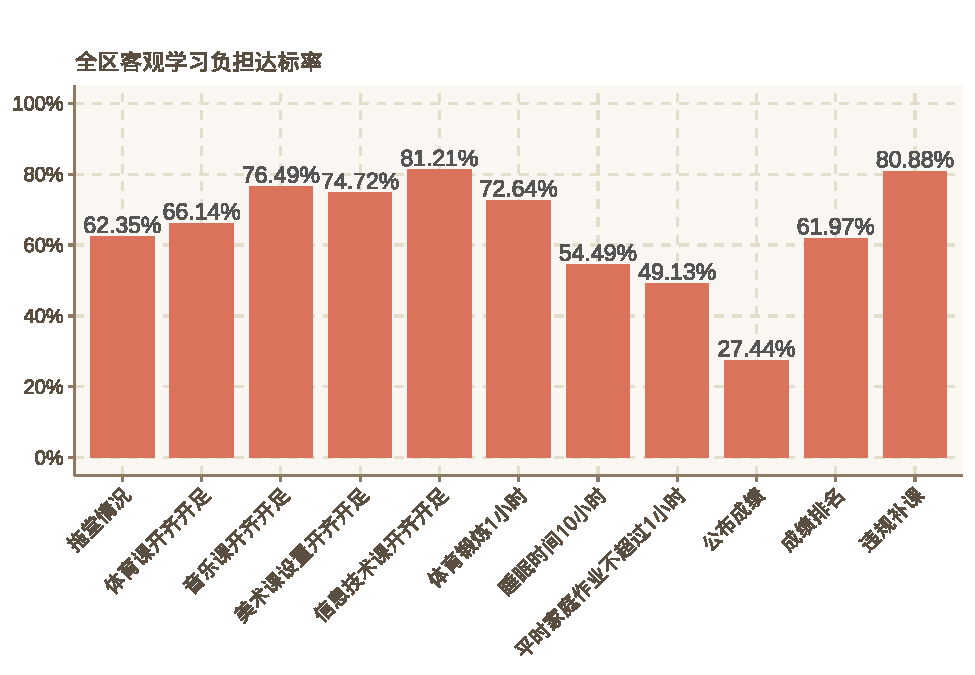
\includegraphics[width=0.95\linewidth]{bookdown_files/figure-latex/unnamed-chunk-13-1} \end{center}

\hypertarget{visul}{%
\chapter{可视化}\label{visul}}

本站《成语故事》收录了五千多个经典成语故事,如八仙过海、画龙点睛、守株待兔、一箭双雕等,都是我们耳熟能详的。成语故事按成语首字读音顺序排列,以故事形式对成语的出处、典故、含义进行清晰明了的解释,故事通俗易懂、内涵深刻、妙趣无穷,真实地再现了一段段传奇往事和历史遗痕。

\begin{center}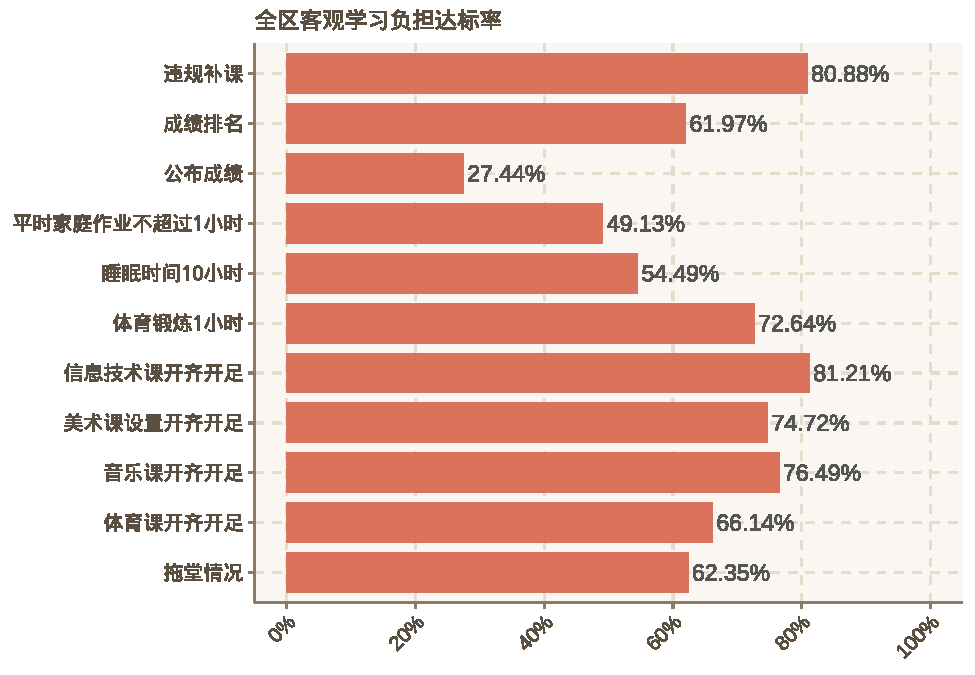
\includegraphics[width=0.95\linewidth]{bookdown_files/figure-latex/unnamed-chunk-14-1} \end{center}

\cleardoublepage

\hypertarget{appendix-ux9644ux5f55}{%
\appendix \addcontentsline{toc}{chapter}{\appendixname}}


\hypertarget{sound}{%
\chapter{工作流程}\label{sound}}

呐,到这里朕的书差不多写完了,但还有几句话要交待,所以开个附录,再啰嗦几句,各位客官稍安勿躁、扶稳坐好。

\hypertarget{ux5916ux90e8ux6587ux4ef6ux7684ux7ed3ux6784}{%
\section{外部文件的结构}\label{ux5916ux90e8ux6587ux4ef6ux7684ux7ed3ux6784}}

需要的清洗和规整

\begin{itemize}
\tightlist
\item
  文件格式csv, 独立于代码文件夹,
\item
  公用的子函数R/也应该独立于代码文件夹
\item
  文件名*.csv用英文、dataframe的列名用英文
\item
  文件规整(group下放 class, school, district)
\item
  如有多个文件合并时(往年数据),确保关键词(学校名)的统一
\item
  题目选择题的选项标签要tidy,需要新建一个表, labels以及断行, 确定出现的字符
\item
  \texttt{forcats::fct\_level}确定label出现的位置顺序
\item
  列的权重,需要新建一个表
\item
  label的需要的规整(小学名称要统一、问卷的题目和选项标签要tidy表\_file2、得分率的权重tidy表\_file3) (2018年的学校名)
\end{itemize}

\hypertarget{ux7a0bux5e8fux7684ux7ed3ux6784ux548cux6d41ux7a0b}{%
\section{程序的结构和流程}\label{ux7a0bux5e8fux7684ux7ed3ux6784ux548cux6d41ux7a0b}}

代码的意图和代码的功能

\begin{itemize}
\item
  统计思路
\item
  将读入的原始数据,mutate必要的(根据问卷直接转换成时间值),形成df\_complete0,
  然后分层summarise()
\item
  df\_complete\_0 人
\item
  df\_complete\_1 班
\item
  df\_complete\_2 校
\item
  df\_complete\_3 区
\item
  school, group, 12个\_percent, 4个mean\_
\item
  最后bind\_rows()堆放一起,方便使用和查询筛选(输入学校名,立马出来这个学校所有的 关结果)
\item
\end{itemize}

\begin{Shaded}
\begin{Highlighting}[]
\NormalTok{    df_all }\OperatorTok\StringTok{ }
\StringTok{     }\KeywordTok{filter}\NormalTok{(school }\OperatorTok{==}\StringTok{ }\NormalTok{set_schoolname ) }\OperatorTok\StringTok{ }
\StringTok{     }\KeywordTok{mutate_at}\NormalTok{(}\KeywordTok{vars}\NormalTok{(}\KeywordTok{ends_with}\NormalTok{(}\StringTok{"_percent"}\NormalTok{)), }
              \KeywordTok{list}\NormalTok{(}\DataTypeTok{RC =} \OperatorTok{~}\NormalTok{. }\OperatorTok{>=}\StringTok{ }\KeywordTok{last}\NormalTok{(.) )}
\NormalTok{              ) }\OperatorTok\StringTok{ }
\StringTok{     }\KeywordTok{mutate}\NormalTok{(}\DataTypeTok{num_above_mean =} \KeywordTok{pmap_dbl}\NormalTok{(}\KeywordTok{select}\NormalTok{(., }\KeywordTok{ends_with}\NormalTok{(}\StringTok{"_percent_RC"}\NormalTok{)), sum)) }\OperatorTok
\StringTok{     }\KeywordTok{select}\NormalTok{(}\OperatorTok{-}\KeywordTok{ends_with}\NormalTok{(}\StringTok{"_percent_RC"}\NormalTok{)) }
\end{Highlighting}
\end{Shaded}

\begin{itemize}
\tightlist
\item
  获得 num\_above\_mean
\item
  school, group, 12个\_percent, 4个mean\_, 1个num\_above\_mean
\item
  可视化
\item
  见 R/function\_all.R
\end{itemize}

\hypertarget{ux7528ux5230ux7684ux6570ux5b66ux65b9ux6cd5lm-ux548cux65b9ux5deeux68c0ux9a8c}{%
\section{用到的数学方法lm 和方差检验}\label{ux7528ux5230ux7684ux6570ux5b66ux65b9ux6cd5lm-ux548cux65b9ux5deeux68c0ux9a8c}}

\begin{itemize}
\tightlist
\item
  关于均值
\item
  本项目,计算的是\textbf{班级的得分}要用\textbf{年级的均值}来比较,\textbf{校的得分}要用\textbf{区的均值}来比较
\item
  因此bind\_row(individual,group),让group的均值放在矢量的\textbf{最后},
\item
  然后mutate(diff = vector - last(vector) )就很方便比较了
\item
  注意不是mutate(diff = vector - mean(vector) )
\end{itemize}

\hypertarget{ux6574ux7406ux641cux7d22ux7684ux4ee3ux7801ux548cux5b8fux5305}{%
\section{整理搜索的代码和宏包}\label{ux6574ux7406ux641cux7d22ux7684ux4ee3ux7801ux548cux5b8fux5305}}

\begin{itemize}
\tightlist
\item
  library(ggthemr)
\item
  颜色不足的时候的ggthemr::swatch
\item
  配色方案网站
\item
  报告模板,如果需要自定义颜色主题,就需要修改模板 latex/preamble.tex
\end{itemize}

\begin{Shaded}
\begin{Highlighting}[]
\NormalTok{% 使用 color=none,需要重重定义下面四种颜色}
\NormalTok
\NormalTok{    \textbackslash{}definecolor\{second\}\{RGB\}\{}\DecValTok{255}\NormalTok{,}\DecValTok{134}\NormalTok{,}\DecValTok{24}\NormalTok{\}% }
\NormalTok{    \textbackslash{}definecolor\{third\}\{RGB\}\{}\DecValTok{0}\NormalTok{,}\DecValTok{0}\NormalTok{,}\DecValTok{0}\NormalTok{\}%}
\end{Highlighting}
\end{Shaded}

\bibliography{book.bib,packages.bib}

\backmatter
\printindex

\end{document}
